\chapter{Equazioni di Maxwell} 

\begin{figure}[h]
    \centering
    \includegraphics{James_Clerk_Maxwell.png}
    
\end{figure}

\begin{figure}[h]
    \centering     
    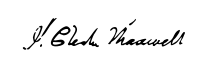
\includegraphics{James_Clerk_Maxwell_sig.png}
    
\end{figure}

\newpage 


\section{Equazioni di Maxwell nel vuoto} 

\footnote{Equazioni di Maxwell - Wikipedia}

Le equazioni di Maxwell sono le seguenti: \\ \\ 

{ \Large \begin{equation}
    \begin{cases}
        
\nabla \cdot \vec{D} = \rho \\ 

\nabla \cdot \vec{B} = 0 \\ 

\nabla \times \vec{E} = -\frac{\partial \vec{B}}{\partial t} \\

\nabla \times \vec{H} = \vec{J} + \frac{\partial \vec{D}}{\partial t}

    \end{cases}
\end{equation}}

\begin{tcolorbox}
    I vettori verranno indicati con la freccia sopra alla lettera del vettore stesso. \\ 
    Un elenco degli operatori matematici che troverai nel corso: \\ \\ 
    
    $\cdot$ Prodotto scalare \\ 
    $\times$ Prodoto vettoriale \\ 
    $\frac{\partial}{\partial t}$ Derivata nel tempo \\ 
    $\nabla$ Operatore nabla \\ 
    $\nabla \cdot$ Divergenza \\  
    $\nabla \times $ Rotore \\ 

    Per capire meglio perchè si usano questi operatori matematici in questo corso, puoi visualizzare questo video di \\\\  
    ClearMath - Rotore e Divergenza: Cosa sono? A che Servono? \\ 
    \url{https://youtu.be/q00XcRm7XBs?si=kWH6J1_2AyCfSYWB} \\\\ 
        
    Step by Step - Fisica e Mate - FISICA Teoria 4 tris - PRODOTTO SCALARE, PRODOTTO VETTORIALE, REGOLA della MANO DESTRA \\ 
    \url{https://youtu.be/MJZnMRb9yZ0?si=rgOIhrHFdt5DQf45} \\\\  


\end{tcolorbox}


Per un vettore F, possiamo visualizzare il rotore e la divergenza come: 


\begin{figure}[h]
    \centering
    \includegraphics[scale= 0.2]{Rotore e Divergenza_ Cosa Sono_ A che Servono_ 1-36 screenshot.png}
    \includegraphics[scale= 0.2]{Rotore e Divergenza_ Cosa Sono_ A che Servono_ 2-10 screenshot.png}
    
\end{figure}

\begin{figure}[h]
    \centering
    \includegraphics[scale= 0.2]{Rotore e Divergenza_ Cosa Sono_ A che Servono_ 6-43 screenshot.png}
    \includegraphics[scale= 0.2]{Rotore e Divergenza_ Cosa Sono_ A che Servono_ 7-6 screenshot.png}
    
\end{figure}

\begin{tcolorbox}
    Le foto sono degli screenshoot da \\
    ClearMath - Rotore e Divergenza: Cosa sono? A che Servono? \\ 
    \url{https://youtu.be/q00XcRm7XBs?si=kWH6J1_2AyCfSYWB} \\\\ 
     
    Da \url{https://it.wikipedia.org/wiki/Divergenza} \\ 
    la divergenza è un campo scalare che misura la tendenza di un campo vettoriale a divergere o a convergere verso un punto dello spazio. \\ 

    Da \url{https://it.wikipedia.org/wiki/Rotore_(matematica)} \\ 
    Il rotore esprime una rotazione infinitesima (ad esempio una velocità di rotazione) del vettore dato, associando a ogni punto dello spazio un vettore.
\end{tcolorbox}
\newpage

\subsection{Legenda - Equazioni di Maxwell nel vuoto}

$\vec{D}$ Flusso del campo elettrico \\ 
$\vec{E}$ Campo elettrico \\ 
$\vec{B}$ Flusso del campo magnetico \\ 
$\vec{H}$ Campo magnetico \\
$\vec{J}$ Densità di corrente \\ 
$\rho$ Densità di carica \\\\ 

\begin{tcolorbox}
    Adesso che sappiamo cosa sono e come si chiamano gli operatori matematici ed i vettori che ci servono, 
    possiamo leggere in italiano le formule matematiche date. \\ 
    
    $\nabla \cdot \vec{D} = \rho$ \\ 
    anche detta legge di Gauss elettrica, esprime che \\ 
    la divergenza del flusso del campo elettrico è uguale alla densità di carica \\ \\

    $\nabla \cdot \vec{B} = 0$ \\ 
    anche detta legge di Gauss magnetica, esprime che \\ 
    la divergenza del flusso del campo magnetico è uguale a zero \\ \\ 

    $\nabla \times \vec{E} = -\frac{\partial \vec{B}}{\partial t}$ \\
    anche detta legge di Faraday, esprime che \\ 
    il rotore del campo elettrico è uguale alla derivata nel tempo del flusso del campo magnetico, 
    con verso contrario rispetto al campo elettrico stesso \\ \\ 
    
    $\nabla \times \vec{H} = \vec{J} + \frac{\partial \vec{D}}{\partial t}$ \newline
    anche detta legge di Ampere-Maxwell, esprime che \\ 
    il rotore del campo magnetico è uguale alla somma della densità di corrente 
    e la derivata nel tempo del flusso del campo elettrico \\ \\ 



\end{tcolorbox}


\newpage 

\section{Equazioni di Maxwell nel vuoto in assenza di cariche} 
\footnote{FWC - pag 132 | 3.9 Maxwell's equations and plane waves}

In assenza di cariche, possiamo considerare: \\

{ \Large \begin{equation}
    \begin{cases}
    
        \rho = 0 \\ 
        \vec{J} = 0  

    \end{cases}
\end{equation}}

\begin{tcolorbox}

    $\rho = 0$ \\
    La densità di carica è uguale a zero \\ \\ 

    $\vec{J} = 0$\\ 
    La densità di corrente è uguale a zero 

\end{tcolorbox}


Quindi, le leggi di Maxwell diventeranno: \\ 


{  \Large \begin{equation}
    \begin{cases}
        \nabla \cdot \vec{D} = \rho \Rightarrow \nabla \cdot \vec{D} = 0  \\
        \nabla \times \vec{H} = \vec{J} + \frac{\partial \vec{D}}{\partial t} 
        \Rightarrow \nabla \times \vec{H} = \frac{\partial \vec{D}}{\partial t} \newline 
        
    \end{cases}
\end{equation}}

Per riassumere, le equazioni di Maxwell nel vuoto in assenza di cariche sono: 

{ \Large \begin{equation}
    \begin{cases}
    
        \nabla \cdot \vec{D} = 0 \\
        \nabla \cdot \vec{B} = 0 \\
        \nabla \times \vec{E} = -\frac{\partial \vec{B}}{\partial t} \\
        \nabla \times \vec{H} = \frac{\partial \vec{D}}{\partial t} \\ 

    \end{cases}
\end{equation}}

\begin{tcolorbox}
    
    $\nabla \cdot \vec{D} = 0$ \\
    La divergenza del flusso del campo elettrico è uguale a zero \\ \\ 

    $\nabla \cdot \vec{B} = 0$ \\
    La divergenza del flusso del campo magnetico è uguale a zero \\ \\ 

    $\nabla \times \vec{E} = -\frac{\partial \vec{B}}{\partial t}$ \\
    Il rotore del campo elettrico è uguale alla derivata nel tempo del flusso del campo magnetico, 
    con verso contrario rispetto al campo elettrico stesso \\ \\ 

    $\nabla \times \vec{H} = \frac{\partial \vec{D}}{\partial t}$ \\ 
    Il rotore del campo magnetico è uguale alla derivata nel tempo del flusso di campo elettrico 

\end{tcolorbox} 

\newpage 

\section{Equazioni di Maxwell nei materiali} 

\footnote{FWC - pag 126 | 3.6 Maxwell's equations in differntial form} 

In questa sezione, prenderemo in considerazione materiali lineari isotropici:
lineari perchè le grandezze del materiale sono lineari, 
isotropici perchè le caratteristiche del materiale 
sono uguali in ogni punto del materiale stesso. \\ 

Ponendo: 

{ \Large \begin{equation}
    \begin{cases}
        
        \varepsilon = \varepsilon_0 \varepsilon_r \\ 
        \mu = \mu_0 \mu_r 

    \end{cases}
\end{equation}} 

$\varepsilon_0$ è la costante dielettrica nel vuoto \\ 
$\varepsilon_r$ è il rapporto tra la costante dielelttrica nel materiale e $\varepsilon_0$ \\ 

$\mu_0$ è la costante di permeabilità nel vuoto \\ 
$\mu_r$ è il rapporto tra la costante di permeabilità nel materiale e $\mu_0$ \\ \\ 

Dalle leggi di Maxwell nel vuoto senza cariche, poniamo: 

{ \Large \begin{equation}
    \begin{cases}
        
        \vec{D} = \varepsilon \vec{E} \\ 
        \vec{B} = \mu \vec{H}

    \end{cases}
\end{equation}} 

\begin{tcolorbox}

    Nota matematica: \\  
    $\varepsilon \vec{E}$ è un prodotto scalare tra uno scalare (quindi un valore) e un vettore. \\ 
    Lo stesso principio vale per $\mu \vec{H}$ \\  

    Nota lettura italiano: \\ \\  
    $\vec{D} = \varepsilon \vec{E}$ \\ 
    Il flusso del campo elettrico è uguale alla costante dielettrica nel materiale per il campo elettrico \\ \\ 

    $\vec{B} = \mu \vec{H}$ \\ 
    Il flusso del campo magnetico è uguale alla costante magnetica nel materiale per il campo magentico 



\end{tcolorbox}


Svolgendo le dovute sostituzioni dalle leggi di Maxwell nel vuoto senza cariche, avremo che: \\ \\ 


{
    \Large 
    \begin{equation}
        \begin{cases}
         \nabla \cdot \vec{D} = 0 
\Rightarrow 
\nabla \cdot (\varepsilon \vec{E}) = 0
\Rightarrow
\nabla \cdot \frac{\varepsilon \vec{E}}{\varepsilon} = \frac{0}{\varepsilon}
\Rightarrow
\nabla \cdot \vec{E} = 0 \\
\nabla \cdot \vec{B} = 0 
\Rightarrow
\nabla \cdot (\mu \vec{H}) = 0
\Rightarrow
\nabla \cdot \frac{\mu \vec{H}}{\mu} = \frac{0}{\mu}
\Rightarrow
\nabla \cdot \vec{H} = 0 \\ 
\nabla \times \vec{E} = -\frac{\partial \vec{B}}{\partial t}
\Rightarrow
\nabla \times \vec{E} = -\frac{\partial (\mu \vec{H} )}{\partial t}
\Rightarrow
\nabla \times \vec{E} = -\mu \frac{\partial \vec{H}}{\partial t}\\ 
\nabla \times \vec{H} = \frac{\partial \vec{D}}{\partial t}
\Rightarrow
\nabla \times \vec{H} = \frac{\partial (\varepsilon \vec{E})}{\partial t}
\Rightarrow
\nabla \times \vec{H} = \varepsilon \frac{\partial \vec{E}}{\partial t}   
        \end{cases}
    \end{equation}
}

Per riassumere, le equazioni di Maxwell nei materiali, in assenza di cariche, sono: 

{ \Large \begin{equation}
    \begin{cases}
        
        \nabla \cdot \vec{E} = 0 \\ \\ 
        \nabla \cdot \vec{H} = 0 \\ \\ 
        \nabla \times \vec{E} = -\mu \frac{\partial \vec{H}}{\partial t} \\ \\ 
        \nabla \times \vec{H} = \varepsilon \frac{\partial \vec{E}}{\partial t} 


    \end{cases}
\end{equation}} 

\begin{tcolorbox}
    $\nabla \cdot \vec{E} = 0 $\\ 
    La divergenza del campo elettrico è uguale a zero \\ \\ 

    $\nabla \cdot \vec{H} = 0$ \\
    La divergenza del campo magnetico è uguale a zero \\ \\ 
    
    $\nabla \times \vec{E} = -\mu \frac{\partial \vec{H}}{\partial t}$ \\  
    Il rotore del campo elettrico è uguale al prodotto tra la derivata del campo magnetico nel tempo per la costante di permeabilità 
    nel materiale con segno opposto rispetto al campo elettrico \\ \\ 

    $\nabla \times \vec{H} = \varepsilon \frac{\partial \vec{E}}{\partial t}$ \\ 
    Il rotore del campo magnetico è uguale al prodotto tra la derivata nel tempo del campo elettrico e la costante elettrica nel materiale



\end{tcolorbox} 

\newpage 
\section{Equazioni di Maxwell nelle coordinate cartesiane} 

\footnote{FWC - pag 85 | 2.5 The curl of a  vector field \\ FWC - pag 132 | 3.9 Maxwell's equations and plane waves } 


Considerando il sistema delle coordinte cartesiane, cioè un sistema in cui ogni punto ha coordinate (x,y,z) , possiamo scrivere che: \\ 

{
    \Large 
    \begin{equation}
 \nabla = (\frac{\partial}{\partial x} , \frac{\partial}{\partial y} , \frac{\partial}{\partial z})
    \end{equation}
}

Quindi: \\ 

{
    \Large
    \begin{equation}
        \nabla \times \vec{E} = \operatorname{rot} 
\begin{vmatrix}
    \hat{x} & \hat{y} &\hat{z} \\ \\ 
    \frac{\partial}{\partial x} & \frac{\partial}{\partial y} & \frac{\partial}{\partial z} \\ \\ 
    E_x & E_y & E_z
\end{vmatrix}  
    \end{equation}
}

$\hat{x} , \hat{y} , \hat{z}$ sono i versori delle coordinate cartesiane, cioè i vettori unitari del sistema cartesiano. \\ 
$E_x , E_y , E_z$ sono le ampiezze di $\vec{E}$ nei rispettivi assi cartesiani \\ 

%Vedi appunti%

Ora andiamo a calcalore il rotore di $\vec{E}$ 

\begin{tcolorbox}
    A livello operativo, calocare il rotore di un vettore significa calcolare il determinante della matrice 
    $\begin{vmatrix}
        \hat{x} & \hat{y} &\hat{z} \\ \\ 
        \frac{\partial}{\partial x} & \frac{\partial}{\partial y} & \frac{\partial}{\partial z} \\ \\ 
        E_x & E_y & E_z
    \end{vmatrix} $ \\ \\ 

    Se non sai calcolare il determinante di una matrice, ti consiglio questo video: \\ \\ Elia Bombardelli - Determinante di una Matrice  \\ \url{https://youtu.be/pstBLN4gCqE?si=pkqB5MmdOgCFapP9} 
\end{tcolorbox}

Svolgendo i calcoli passo-passo, avremo che: \\ 

{
    \Large
    \begin{equation}
        \begin{split}
        \nabla \times \vec{E} 
        &= \operatorname{rot} 
\begin{vmatrix}
    \hat{x} & \hat{y} &\hat{z} \\ \\ 
    \frac{\partial}{\partial x} & \frac{\partial}{\partial y} & \frac{\partial}{\partial z} \\ \\ 
    E_x & E_y & E_z
\end{vmatrix}  \\ \\
&= \hat{x} 
\begin{vmatrix}
    \frac{\partial}{\partial y} & \frac{\partial}{\partial z} \\  \\ 
    E_y & E_z 
\end{vmatrix}  
- \hat{y} 
\begin{vmatrix}
    \frac{\partial}{\partial x} & \frac{\partial}{\partial z} \\  \\ 
    E_x & E_z 
\end{vmatrix} 
+ \hat{z} 
\begin{vmatrix}
    \frac{\partial}{\partial x} & \frac{\partial}{\partial y} \\  \\ 
    E_x & E_y 
\end{vmatrix} \\ \\
&= \hat{x} (\frac{\partial E_z}{\partial y} - \frac{\partial E_y}{\partial z})
 - \hat{y} (\frac{\partial E_z}{\partial x} - \frac{\partial E_x}{\partial z})
 + \hat{z} (\frac{\partial E_y}{\partial x} - \frac{\partial E_x}{\partial y}) \\ \\
&= \hat{x} (\frac{\partial E_z}{\partial y} - \frac{\partial E_y}{\partial z})
 + \hat{y} (-\frac{\partial E_z}{\partial x} + \frac{\partial E_x}{\partial z})
 + \hat{z} (\frac{\partial E_y}{\partial x} - \frac{\partial E_x}{\partial y})
        \end{split}
    \end{equation}
}

Possiamo svolgere gli stessi passaggi svolti anche per $\nabla \times \vec{H}$ \\

{
    \Large
    \begin{equation}
\nabla \times \vec{H} 
= \hat{x} (\frac{\partial H_z}{\partial y} - \frac{\partial H_y}{\partial z})
+ \hat{y} (-\frac{\partial H_z}{\partial x} + \frac{\partial H_x}{\partial z})
+ \hat{z} (\frac{\partial H_y}{\partial x} - \frac{\partial H_x}{\partial y})
    \end{equation}
}

Per riassumere, le equazioni di Maxwell nei materiali nelle coordinate cartesiane sono le seguenti: \\ 

{ \Large \begin{equation}
    \begin{cases}
        \nabla \cdot \vec{E} = 0 \\ \\ 
        \nabla \cdot \vec{H} = 0 \\ \\
        
        \nabla \times \vec{E} 
        = \hat{x} (\frac{\partial E_z}{\partial y} - \frac{\partial E_y}{\partial z})
        + \hat{y} (-\frac{\partial E_z}{\partial x} + \frac{\partial E_x}{\partial z})
        + \hat{z} (\frac{\partial E_y}{\partial x} - \frac{\partial E_x}{\partial y}) \\ \\ 


        \nabla \times \vec{H}  
 = \hat{x} (\frac{\partial H_z}{\partial y} - \frac{\partial H_y}{\partial z})
 + \hat{y} (-\frac{\partial H_z}{\partial x} + \frac{\partial H_x}{\partial z})
 + \hat{z} (\frac{\partial H_y}{\partial x} - \frac{\partial H_x}{\partial y}) \\ 


 
    \end{cases}
\end{equation}} 

\newpage 

\section{Equazioni di Maxwell per le onde piane in (x, y, z)}
\footnote{FWC - pag 132 | 3.9 Maxwell's equations and plane waves }


Considerando le onde piane, cioè onde in cui il fronte d'onda è infinito, possiamo calcolarci le equazioni di Maxwell per questo 
tipo d'onda. \\ 

Le onde piane, nella realtà, non esistono, ma ci sono utili per modellare le onde reali e per semplificarci i conti:
da sei incognite delle equazioni di Maxwell trovate nella sezione precedente, passeremo a due, cioè $E_x$ e $E_y$. \\ 
Gli altri componenti del campo elettromagnetico dipenderanno da queste due variabili indipendenti. \\ 


Ricordando che il fronte d'onda è infinito, 
le onde piane sono onde per cui non c'è variazione dell'onda lungo l'asse x e lungo l'asse y, quindi possiamo scrivere: 

{ \Large \begin{equation}
    \begin{cases}
        \frac{\partial}{\partial x} = 0 \\ \\  
        \frac{\partial}{\partial y} = 0 \\ 
        
    \end{cases}
\end{equation}}

$\nabla \times \vec{E}$ da: 

{
    \Large
    \begin{equation}
        \nabla \times \vec{E} 
        = \hat{x} (\frac{\partial E_z}{\partial y} - \frac{\partial E_y}{\partial z})
        + \hat{y} (-\frac{\partial E_z}{\partial x} + \frac{\partial E_x}{\partial z})
        + \hat{z} (\frac{\partial E_y}{\partial x} - \frac{\partial E_x}{\partial y}) 
    \end{equation}
}

diventa: 

{
    \Large 
    \begin{equation}
        \nabla \times \vec{E} = \hat{x} (- \frac{\partial E_y}{\partial z})
+ \hat{y} (\frac{\partial E_x}{\partial z})
+ \hat{z} (0)  
    \end{equation}
}

Dalle leggi di Maxwell nei materiali, sappiamo che:  

{
    \Large 
    \begin{equation}
        \nabla \times \vec{E} = - \mu \frac{\partial \vec{H}}{\partial t}   
    \end{equation}
}

Scomponendo questa equazione nei vari assi cartesiani, avremo che: \\ \\ 

\textbf{Asse X} 
{
    \Large
    \begin{equation}
     -\frac{\partial E_y}{\partial z} = -\mu \frac{\partial H_x}{\partial t}   
    \end{equation}
}

\textbf{Asse Y}  

{
    \Large
    \begin{equation}
        \frac{\partial E_x}{\partial z} = -\mu \frac{\partial H_y}{\partial t}  
    \end{equation}
}

\textbf{Asse Z}  

{
    \Large 
    \begin{equation}
        0 = -\mu \frac{\partial H_z}{\partial t}   
    \end{equation}
}

Quello che abbiamo fatto per $\nabla \times \vec{E}$, possiamo farlo anche per $\nabla \times \vec{H}$ \\ 

{
    \Large
    \begin{equation}
     \nabla \times \vec{H} = \varepsilon \frac{\partial \vec{E}}{\partial t}   
    \end{equation}
}
Scomponendo questa equazione nei vari assi cartesiani, avremo che: \\ \\ 

\textbf{Asse X} 
{
    \Large 
    \begin{equation}
    -\frac{\partial H_y}{\partial z} = \varepsilon \frac{\partial E_x}{\partial t}   
    \end{equation}
}

\textbf{Asse Y} 
{
    \Large 
    \begin{equation}
     \frac{\partial H_x}{\partial z} = \varepsilon \frac{\partial E_y}{\partial t}   
    \end{equation}
}


\textbf{Asse Z} 
{
    \Large
    \begin{equation}
        0 = \varepsilon \frac{\partial E_z}{\partial t}    
    \end{equation}
}

\begin{tcolorbox}
    Scriverò un esempio che può essere applicato per tutte le altre eqazioni. \\ \\ 
    $\frac{\partial H_x}{\partial z} = \varepsilon \frac{\partial E_y}{\partial t}$ \\ 

    La derivata per z della componente sull'asse x del campo magnetico è uguale al prodotto tra la costante elettrica nel materiale e la derivata 
    nel tempo della componente sull'asse y del campo elettrico 

\end{tcolorbox}

Considerando le equazioni sull'asse z, abbiamo che: \\ 

{ \Large \begin{equation}
    \begin{cases}
        \varepsilon \frac{\partial E_z}{\partial t} = 0 \\
        -\mu \frac{\partial H_z}{\partial t} = 0 
    \end{cases} 
    \Rightarrow
    \begin{cases}
        E_z = 0\\
        H_z = 0 
    \end{cases}
\end{equation}} \\ 

Queste equazioni ci dicono che i campi sono trasversali rispetto alla direzione di propagazione (considerando 
l'asse z come asse di propagazione)

\begin{tcolorbox}
    Da \url{https://it.wikipedia.org/wiki/Onda_trasversale} \\
    Un' onda trasversale è un'onda in movimento che è composta da oscillazioni che avvengono perpendicolari alla direzione del trasferimento di energia. Se un'onda trasversale si muove nella direzione positiva x, le sue oscillazioni sono nelle direzioni sopra e sotto che giacciono nel piano y-z.
\end{tcolorbox}

Questo significa che $\vec{E}$ e $\vec{H}$ sono perpendicolari. 

Analizzando le altre equazioni nel piano (x,y), notiamo che: 

{ \Large \begin{equation}
    \begin{cases}
        \frac{\partial E_x}{\partial z} = -\mu \frac{\partial H_y}{\partial t} \\
        -\frac{\partial H_y}{\partial z} = \varepsilon \frac{\partial E_x}{\partial t} 

    \end{cases}
\end{equation}} \\ 

Possiamo risolvere questo sistema per $E_x$ \\ 

Differenziando per $\frac{\partial}{\partial z}$ nella prima equazione e $\frac{\partial}{\partial t}$ 
nella seconda equazione, avremo che: 

{ \Large \begin{equation}
    \begin{cases}
        \pdv[2]{E_x}{z} = - \mu \pdv{H_y}{t}{z} \\ \\  
        \pdv[2]{H_y}{z}{t} = - \mu \pdv{E_y}{t} \\ 
        
    \end{cases}
\end{equation}} \\ 

Sostituendo la seconda equazione alla prima, abbiamo che: \\ \\ 

{
    \Large 
    \begin{equation}
        \pdv[2]{E_x}{z} = \mu \varepsilon \pdv[2]{E_x}{t}   
    \end{equation}
}

Questa indicata è l'equazione dell'onda a una dimensione lunga la direzione z. 

Lo stesso procedimento svolto per trovare $E_x$, lo possiamo usare con $E_y$ \\ 

L'onda si propaga con velocità: \\ \\ 

{
    \Large
    \begin{equation}
        v = \frac{1}{\sqrt{\mu \varepsilon}}
    \end{equation}
}

\begin{tcolorbox}
    Per vedere un altro punto di vista dell'equazione dell'onda, puoi visualizzare questo video di \\ \\
    Ali the Dazzling - The Wave Equation simplified \\ 
    \url{https://youtu.be/tGc4gb8n7gM?si=H4Jw0vzIKAW2jeqv} \\ 

    Putroppo è in inglese e non ha i sottotitoli in italiano, ma il video è molto semplice e molto intuitivo 
\end{tcolorbox}

\newpage 

\section{Equazioni di Maxwell in forma fasoriale}
\footnote{FWC - pag 135 | 3.10 Uniform plane waves with steady-state sinusoids}

Oltre alle onde piane negli assi cartesiani, è possibile esprimere le onde usando i fasori. 

\begin{tcolorbox}
    Se non sai cosa è un fasore, puoi visualizzare questo video di \\ \\ 
    Elettronica-mente - Elettrotecnica - Lezione 15 - Fasori, Impedenza ed Ammettanza \\ 
    \url{https://youtu.be/_Yww5MfoPwI?si=7e-8G0q_gUFOcTev} 

\end{tcolorbox}

Ponendo: 
{
    \Large
    \begin{equation}
    \frac{\partial}{\partial t} = \jmath \omega   
    \end{equation}
}

possiamo riscrivere le equazioni di Maxwell nei materiali come: \\   

{ \Large \begin{equation}
    \begin{cases}
        \nabla \cdot \vec{D} = 0 \\
        \nabla \cdot \vec{B} = 0 \\
        \nabla \times \vec{E} = -\mu \frac{\partial \vec{H}}{\partial t} \\
        \nabla \times \vec{H} = \varepsilon \frac{\partial \vec{E}}{\partial t}  

    \end{cases} 
    \Rightarrow
    \begin{cases}
        \nabla \cdot \vec{D} = 0 \\
        \nabla \cdot \vec{B} = 0 \\
        \nabla \times \vec{E} = - \jmath \omega \mu \vec{H} \\
        \nabla \times \vec{H} = \jmath \omega \varepsilon \vec{E}  

    \end{cases}
\end{equation}} \\ 


Per lo stesso principio, possiamo scrivere le sue componenti lungo (x,y, z) come: \\ 

{
    \Large 
    \begin{equation}
    \nabla \times \vec{E} = - \jmath \omega \mu \vec{H}    
    \end{equation}
}

\textbf{Asse X} 

{
    \Large 
    \begin{equation}      
-\frac{\partial E_y}{\partial z} = -\jmath \omega \mu H_x 
    \end{equation}
}

\textbf{Asse Y}  
{
    \Large
    \begin{equation}
\frac{\partial E_x}{\partial z} = - \jmath \omega \mu H_y    
    \end{equation}
}

\textbf{Asse Z} 
{
    \Large
    \begin{equation}
        0 = \jmath \omega \mu H_z   
    \end{equation}
}

Invece per: 

{
    \Large
    \begin{equation}
    \nabla \times \vec{H} = \jmath \omega \varepsilon \vec{E} 
    \end{equation}
}

\textbf{Asse X} 
{
    \Large 
    \begin{equation}
        -\frac{\partial H_y}{\partial z} = \jmath \omega \varepsilon E_x   
    \end{equation}
} 


\textbf{Asse Y} 
{
    \Large
    \begin{equation}
    \frac{\partial H_x}{\partial z} = \jmath \omega \varepsilon E_y   
    \end{equation}
}

\textbf{Asse Z} 

{
    \Large
    \begin{equation}
    0 = \jmath \omega \varepsilon E_z  
    \end{equation}
}
L'equazione dell'onda, in forma fasoriale, diventa: \\ 

{
    \Large
    \begin{equation}
    \pdv[2]{E_x}{z} = - \omega ^ 2 \mu \varepsilon E_x   
    \end{equation}
}

in cui 

{
    \Large
    \begin{equation}
        \pdv[2]{}{t} = - \omega ^ 2   
    \end{equation}
}
in forma fasoriale. 

Come il caso delle equazione di Maxwell delle onde onde piane nei materiali, 
{
    \Large
    \begin{equation}
E_z = H_z = 0 
    \end{equation}
}
\newpage 









